\section{Autoencoders}

\subsection{Part 1: Constructing the Autoencoder} 
    
The training curve is given below:


% Training curve
 \begin{figure}[H]
   \centering
     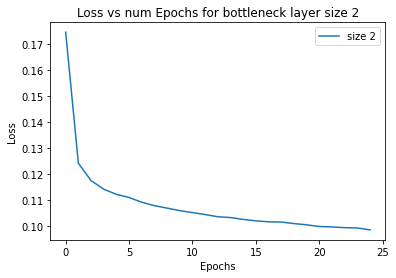
\includegraphics[scale=0.8]{templates/ae_curve1}
 \end{figure}

The reconstructions of the last minibatch for epochs 0, 10, and 20 are:


% Epoch 0
 \begin{figure}[H]
   \centering
     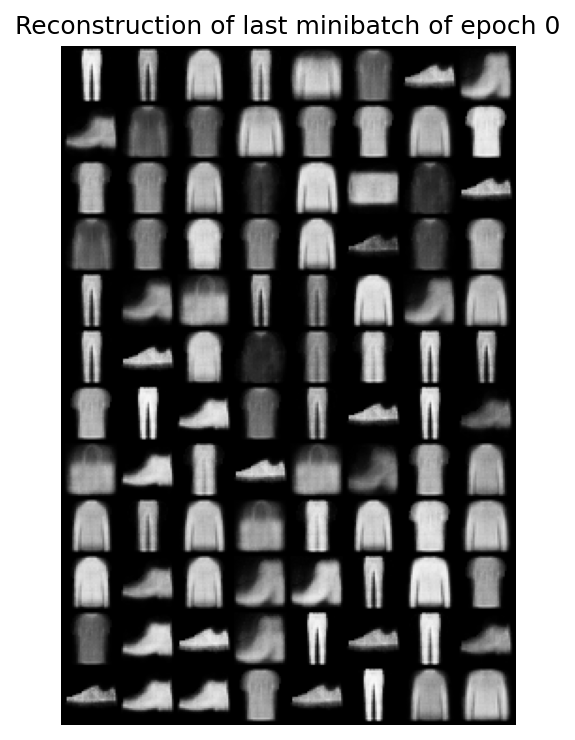
\includegraphics[scale=0.8]{templates/re0}
 \end{figure}

% Epoch 10
 \begin{figure}[H]
   \centering
     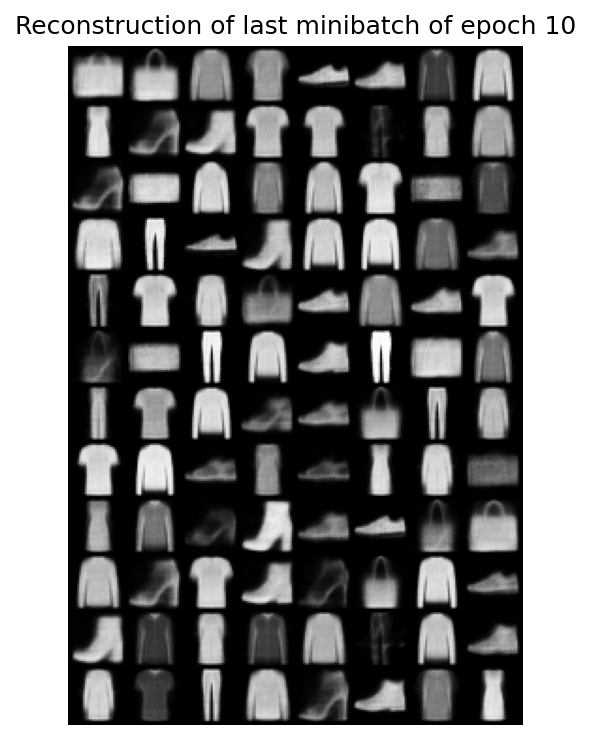
\includegraphics[scale=0.8]{templates/re10}
 \end{figure}

% Epoch 20
 \begin{figure}[H]
   \centering
     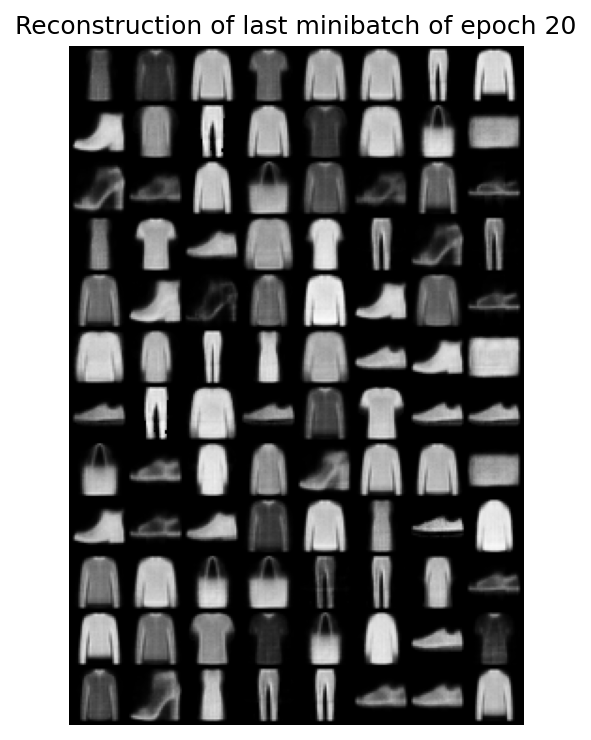
\includegraphics[scale=0.8]{templates/re20}
 \end{figure}


\subsection{Part 2: Latent Space Decomposition }
\begin{enumerate}
    \item Plot of the latent space of this autoencoder:
    
    Changed random seed to 40 to get a better latent space plot since the original one was a vertical line.
    % latent space plot
    \begin{figure}[H]
      \centering
         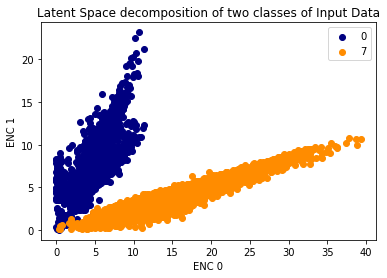
\includegraphics[scale=0.8]{templates/latent1}
    \end{figure}

    \item From the latent space plot, explain what the encoding has done to the inputs. How is this effect related to what PCA does? Why is this useful?
    \newline\newline
    The latent space is where encoded vectors lie. The encoder decreases the dimensionality of the input up to the latent space. PCA is looking for the best linear subspace of the initial space described by an orthogonal basis of new features such that the error of approximating the data by their projections on this subspace is as small as possible. 
	\newline \newline
	PCA and the Encoder are similar in that both are building new features using the features of the input dataset. The capability to compress data can be used for a variety of tasks such as removing noise / occlusions from images, developing lossy compression algorithms and machine translation.

\end{enumerate}

\subsection{Part 3: Reconstruction Error vs Bottleneck Layer} 
\begin{enumerate}
    \item Report the combined training curves (mean epoch loss vs epochs) for all the bottleneck layer sizes $[2,8,32,64]$. Also report the reconstructed images for Epoch 20 for each of the configurations.
    
    The training curves of all the configurations:

    % training curve plot
     \begin{figure}[H]
       \centering
         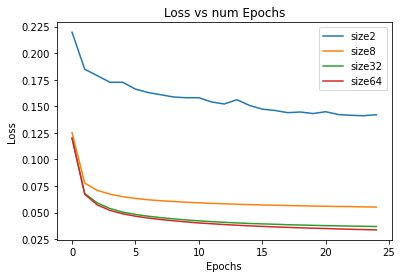
\includegraphics[scale=0.8]{templates/loss1}
     \end{figure}

The reconstructions for sizes $[2,8,32,64]$ for epoch 20 of the last minibatch:

% bottleneck 2
 \begin{figure}[H]
   \centering
     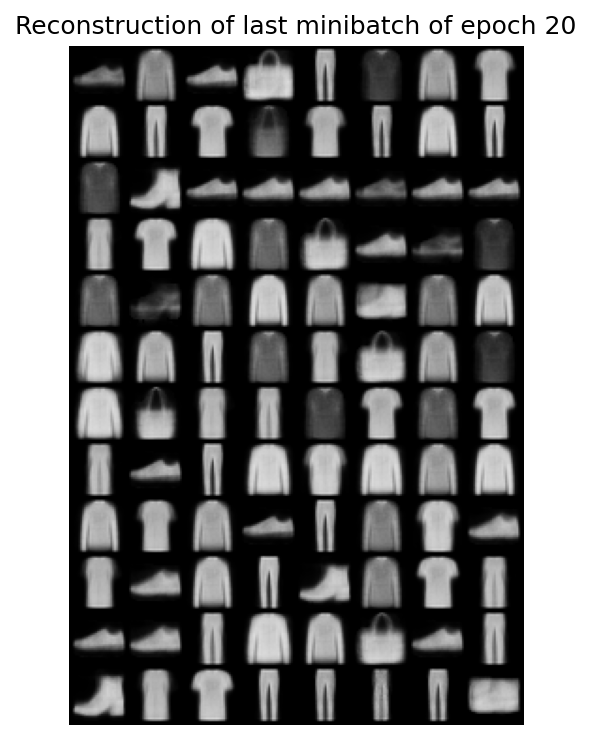
\includegraphics[scale=0.6]
     {templates/re20_2}
     \caption{Size 2}
 \end{figure}

% bottleneck 8
 \begin{figure}[H]
   \centering
     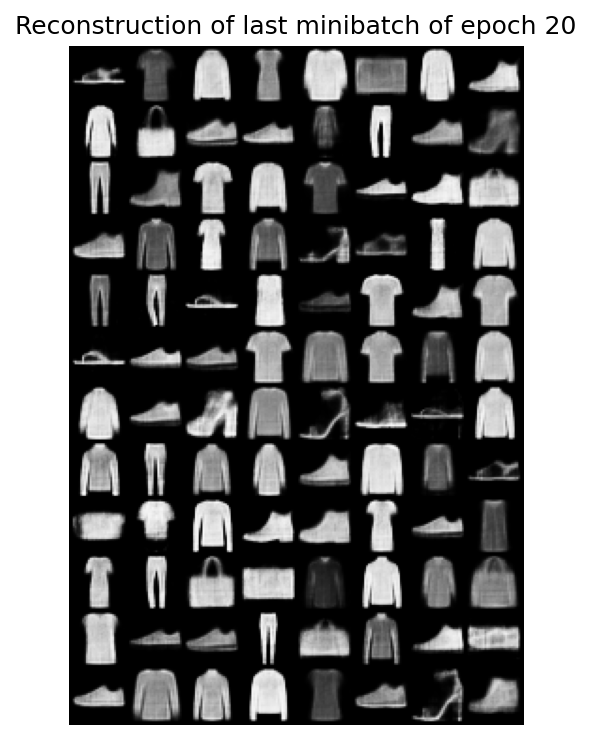
\includegraphics[scale=0.6]
     {templates/re20_8}
     \caption{Size 8}
 \end{figure}

% bottleneck 32
 \begin{figure}[H]
   \centering
     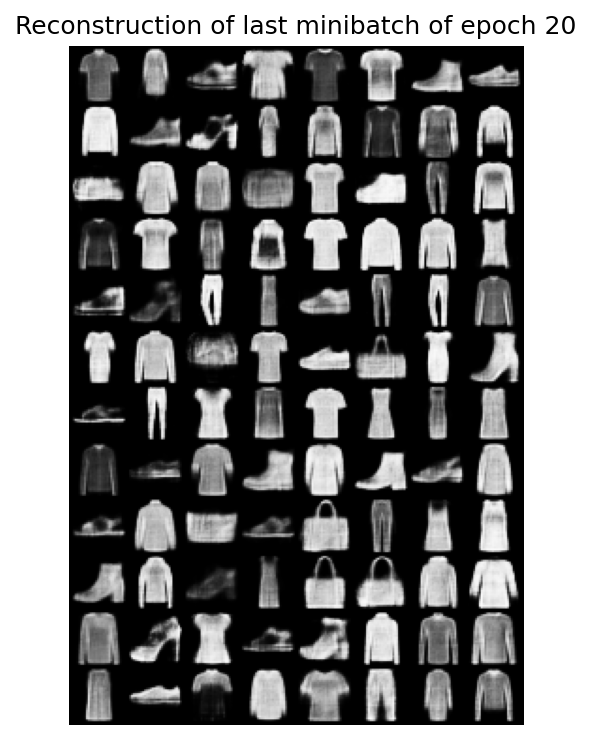
\includegraphics[scale=0.6]
     {templates/re20_32}
     \caption{Size 32}
 \end{figure}

% bottleneck 64
 \begin{figure}[H]
   \centering
     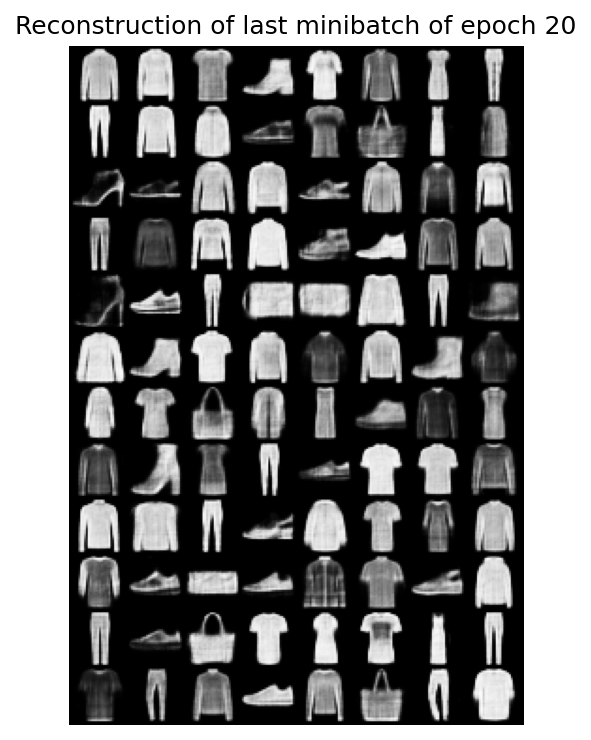
\includegraphics[scale=0.6]
     {templates/re20_64}
     \caption{Size 64}
 \end{figure}


\item 
The reconstruction error for images of class 0 as the bottleneck layer size increases:

% reconstruction vs size
 \begin{figure}[H]
   \centering
     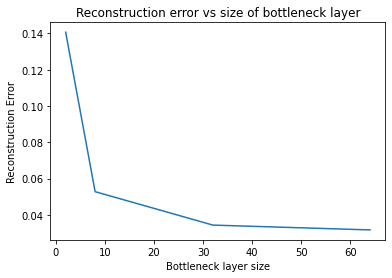
\includegraphics[scale=0.6]
     {templates/reconstruction1}
 \end{figure}

What are you observing? How does what you see relate to PCA? What does this tell you about how you can potentially work with a high-dimensional data-space?
\newline \newline
Observations based on how reconstruction error changes with bottleneck layer size, and similarities to PCA:
\begin{enumerate}
\item Inflection point at the bottleneck layer size of 32, indicating that 32 is the least number of dimensions required for optimally encoding the dataset.
\item Similar to how the PCA analysis helps determine the top $k$ features which account for most of the variance seen in the data, this analysis tells us that 32 features explain most of the variance in this dataset.
\end{enumerate}

Solutions for dealing with high-dimensional data spaces: (a) PCA to generate new features which are linear combinations of input features; (b) In a Vanilla Autoencoder, the latent space forms a bottleneck which forces the model to learn an effective compression of the data.

\end{enumerate}
